\documentclass[../../main.tex]{subfiles}

\begin{document}

\section{LabView II}

\begin{fulltheorem}
  Állapotgép LabVIEW-ban.
\end{fulltheorem}

Az \kix{állapotgép} egy programozási struktúra is. Sok esetben egy programban,
folyamatban vissza kell lépni, vagy lépéseket ki kell hagyni. Ez függhet a
kezelőtől, de lehet az algoritmusba beépített tudás is.

Állapotgép algoritmussal működnek a bankautomaták, mert a folyamatban lehet,
hogy visszalépünk, de a válaszaink, vagy a bankkártyánk típusa miatt egyes
lépések ki is maradhatnak. A pénztárgépek is tudják, hogy kis tételnél, ha
érintős a kártya nem kell PIN kódot kérni, tehát kihagyható ez a lépés.

\subsection{Algoritmus meghatározása}

Először állítsuk össze a tevékenységlistát, és nevezzük el őket.
Határozzuk meg, hogy melyik tevékenységet milyen folyamat követhet.
Készíteni kell egy \cix{enum} konstanst a tevékenységek nevével, valamint egy
\cix{case} struktúrát, amelyet az előzőleg definiált konstans fog vezérelni.
Létre kell hozni minden esethez a \tc{frame}-et, és minden \tc{frame}-ben kell
egy olyan \tc{enum} típusú kimenet, amely a következő végrehajtandó \tc{frame}
nevét tartalmazza. Az egészet körbeveszi egy \cix{while} ciklus egy
\kix{Shift regiszter}[rel]
\begin{figure}[H]
  \centering
  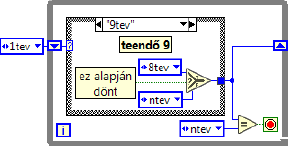
\includegraphics[width=.6\textwidth]{../../static/lw/state-machine.png}
  \caption{Állapotgép LabVIEW-ban}
  \label{fig:lv/sm}
\end{figure}

\paragraph*{Példa}

Készítsunk programot, amely egy oldalhosszaival adott háromszög kerületét
és területét számolja ki egy gomb lenyomása után, de csak akkor, ha az
oldalhosszak megfelelnek a háromszög egyenlőségnek. A lehetséges állapotok:
\begin{multicols}{4}
  \begin{itemize}
    \item vár,
    \item ellenőriz,
    \item számol,
    \item vissza.
  \end{itemize}
\end{multicols}

\end{document}
